\section{VECSEL Chips}\label{sec:vecsel}

TODO: redo design images maybe with legend? different colors?

The basic structure of a VECSEL gain chip is shown in \cref{fig:vecDes}. The main feature of the structure are as follows: 

\begin{itemize}
    \item Heat spreader: The heat spreader role is in dissipating the heat generated during the operation of the VECSEL chip to a Peltier-controlled copper heat-sink.
    \item Pump \& laser  DBR: The purpose of the two bottom mirrors is to reflect the laser light and the pump light. There are two main advantages to this approach: firstly, because of higher absorption, there is a higher optical-to-optical efficiency due to the two passes through the active region, and secondly, there is less absorption in the mirror and in the heat sink, which results also in a higher efficiency and a higher maximum output power. The high reflectivity for two wavelengths is realized by using a distributed Bragg reflector (DBR)
    \item Active region: The purpose of the active region is the conversion of the pump light into the laser light. The gain medium in the active region is often composed of quantum wells or quantum dots.
    \item Anti-reflection coating: The anti-reflection section is optimized to reduce the otherwise large reflection from the air/GaAs interface
\end{itemize}

Below the three different structure of the VECSEL chips used in this work.

\begin{figure}[ht]
    \centering
    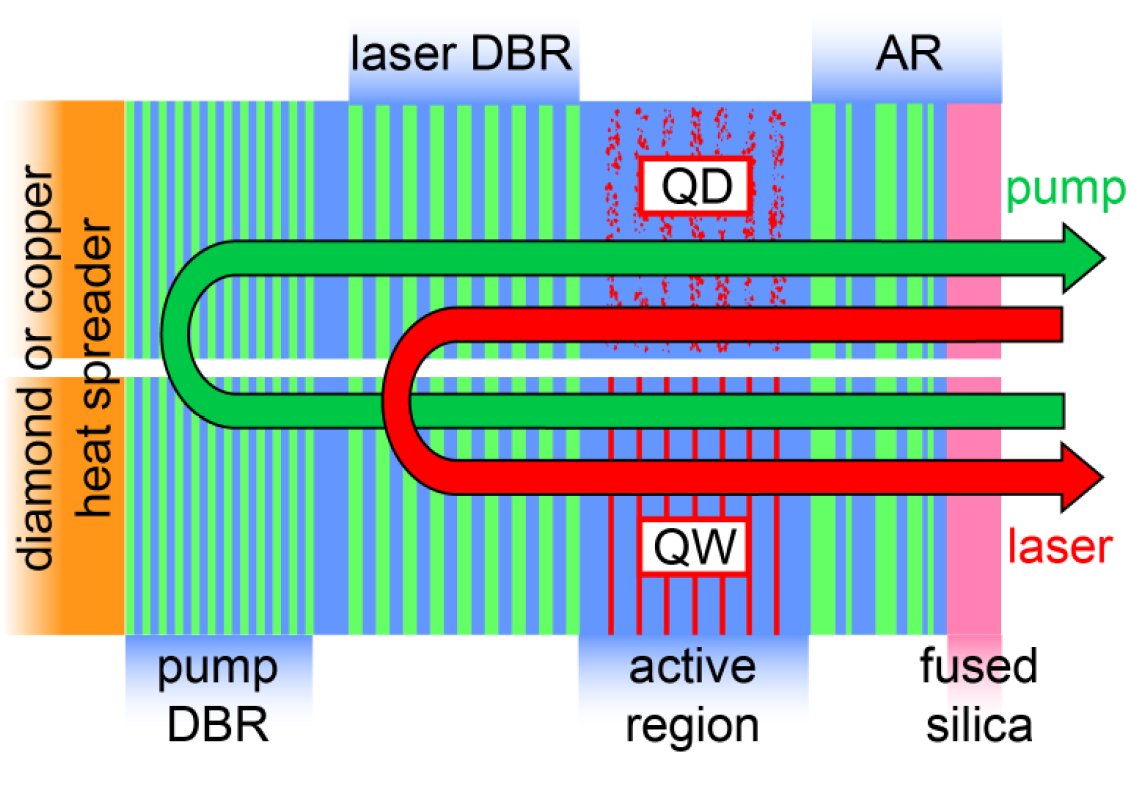
\includegraphics[width=.6\linewidth]{images/VECSEL_structure.png}
    \caption{TODO: caption}
    \label{fig:vecDes}
\end{figure}


%A distributed Bragg reflector (DBR) for the pump wavelength (808 nm) reflects the unabsorbed pump light, reducing heat deposition in the structure and increasing efficiency.
% The DBR for the laser wavelength acts as a flat cavity mirror.


\subsection*{No pump DBR chip, SV166}

\begin{wrapfigure}{r}{.4\textwidth}
    \vspace{-\baselineskip}
    \centering
    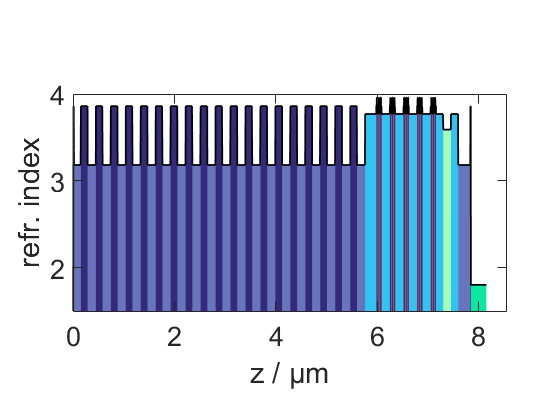
\includegraphics[width=.98\textwidth]{images/1SV166.lay.png}
    \caption{TODO: caption}
    \label{fig:sv166}
\end{wrapfigure}

This structure has an antiresonant design and cooled from the backside by a copper heat spreader. The DBR consists of 19-pairs of GaSb/AlAs\textsubscript{0.08}Sb\textsubscript{0.92} layers design around a wavelength of \qty{2080}{nm}. The active region has $5\times3$ In\textsubscript{0.27}Ga\textsubscript{0.73}Sb quantum wells (QW) placed at the maximum of the standing-wave cavity. Additional barriers layer made of AlAs\textsubscript{0.08}Sb\textsubscript{0.92} are placed around the gain QW to increase the photoluminesence. The last layer is a PECVD coating made of Si\textsubscript{3}N\textsubscript{4}, which serves an an anti-reflection coating.


\subsection*{Pump DBR chip, SV167}

\begin{wrapfigure}{r}{.4\textwidth}
    \vspace{-\baselineskip}
    \centering
    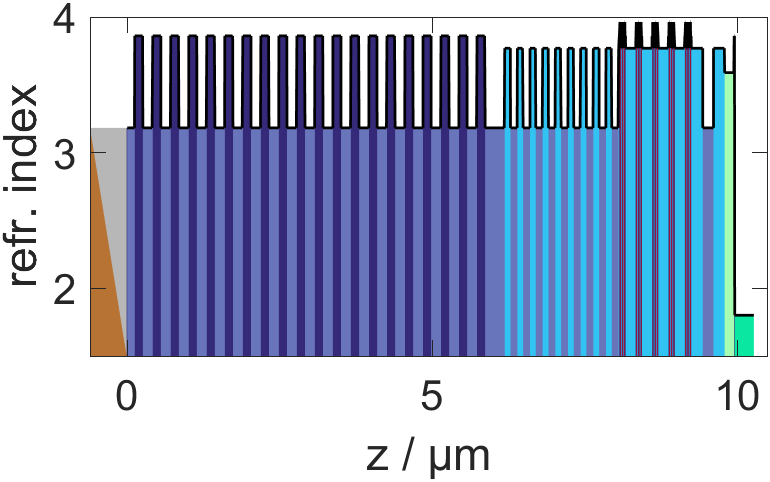
\includegraphics[width=.98\textwidth]{images/1SV167B.lay.png}
    \caption{TODO: caption}
    \label{fig:sv167}
\end{wrapfigure}

This is a similar structure as above but this time including an extra DBR for the pump wavelength of \qty{1470}{\nm}. The pump DBR is made of 10 layers of Al\textsubscript{0.2}As\textsubscript{0.8}Sb/Al\textsubscript{0.15}Ga\textsubscript{0.85}AsSb. For the thickness of the layers the \qty{45}{\degree} incident of the pump beam had to be accounted for. This structure was measured twice but for different heat spreaders, one made of copper and the other of diamond, to observe and compare the influence of better thermal conductivity of the heat spreader.


\subsection*{Hybrid chip, SV165}

\begin{wrapfigure}{r}{.4\textwidth}
    \vspace{-\baselineskip}
    \centering
    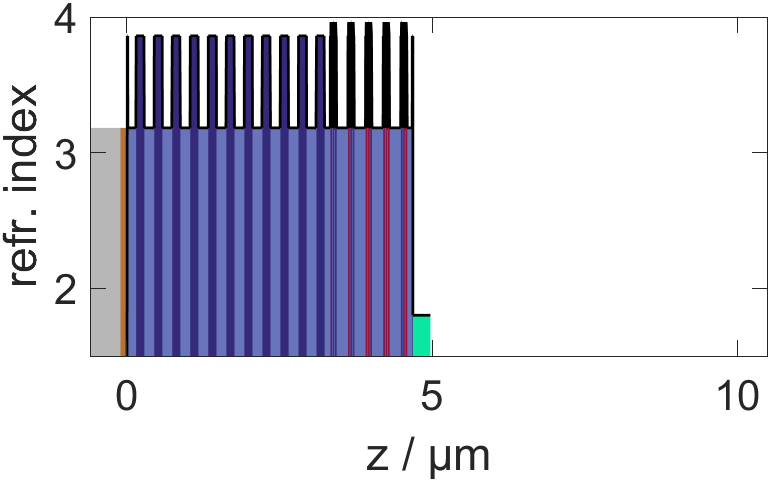
\includegraphics[width=.98\textwidth]{images/1SV165.lay.png}
    \caption{TODO: caption}
    \label{fig:sv165}
\end{wrapfigure}

This structure incorporated a hybrid metal-semiconductor Bragg reflector. It consisted of a  \qty{100}{\nm} copper layer with 10.5 AlAs\textsubscript{0.08}Sb\textsubscript{0.92}/GaSb layers. This allows for a thinner gain chip design of just under \qty{5}{\um} compared to the other structures \qty{7.5}{\um} resp. \qty{10}{\um} for the pump DBR design. This lowered the thermal resistance of the device by \qty{24}{\percent}. This structure also has a different active region made of $5\times3$ In\textsubscript{0.27}Ga\textsubscript{0.73}Sb/GaSb QW.